\chapter{Genres, instruments and tools}

\section{Genres}\label{genres}

Before starting to write an electroacoustic piece we should:

\begin{itemize}
\tightlist
\item define the instrumentation to be used which can include acoustic instruments, electroacoustic instruments, virtual instruments or a mix of these types.
\item define the sound amplification and diffusion system.
\end{itemize}

%\begin{center}
%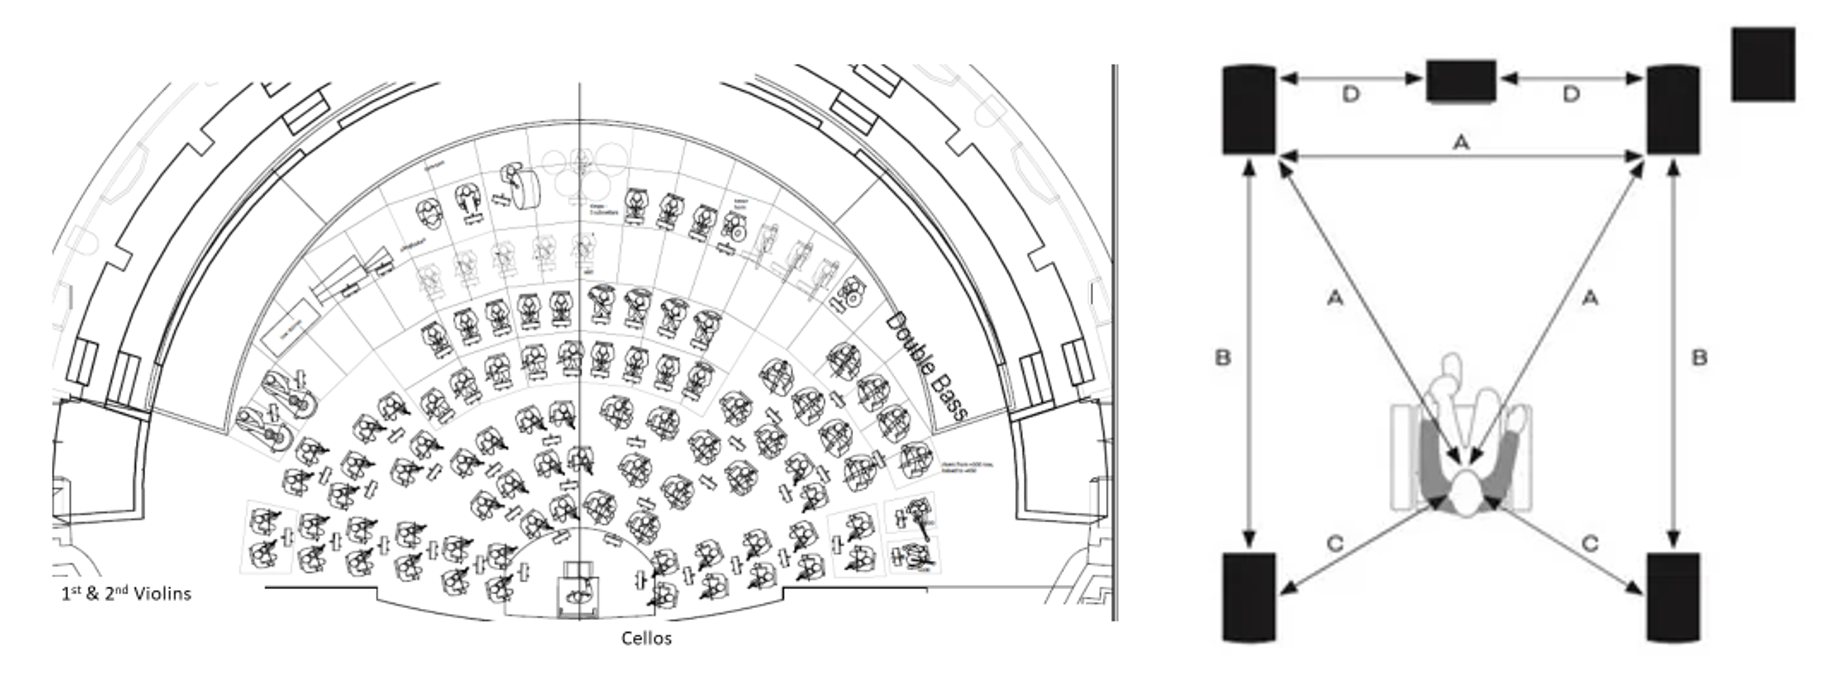
\includegraphics[scale=0.9]{img/dispo.png}
%\end{center}

For this reason here we categorize the different types and genres of electroacoustic music by dividing them into two macro areas defined by the way of controlling sounds and musical parameters.

\begin{itemize}
\tightlist
\item non interactive systems.
\item interactive systems.
\end{itemize}

We will explore the compositional strategies of each in dedicated chapters.

\section{Non interactive systems}\label{non-interactive-systems}

This category includes genres that:

\begin{itemize}
\tightlist
\item don't involve any human interaction during the performance.
\item involve interactions that don't influence the musical or sound text in any way.
\end{itemize}

According with the reflections of the previous chapter we can affirm:

\begin{itemize}
\tightlist
\item interactions may influence the listener's perception of the sound text (mainly through the different characteristics of the diffusion systems used).
\item interactions don't change the sound text.
\end{itemize}

This category can be divided into two further subcategories:

\begin{itemize}
\tightlist
\item fixed media music.
\item live sequencing.
\end{itemize}

The image shows the possibles audio chains in this category.

\begin{itemize}
\tightlist
\item non-real-time sound processing.
\item non-real-time synthesis.
\item real-time synthesis.
\end{itemize}

\begin{center}
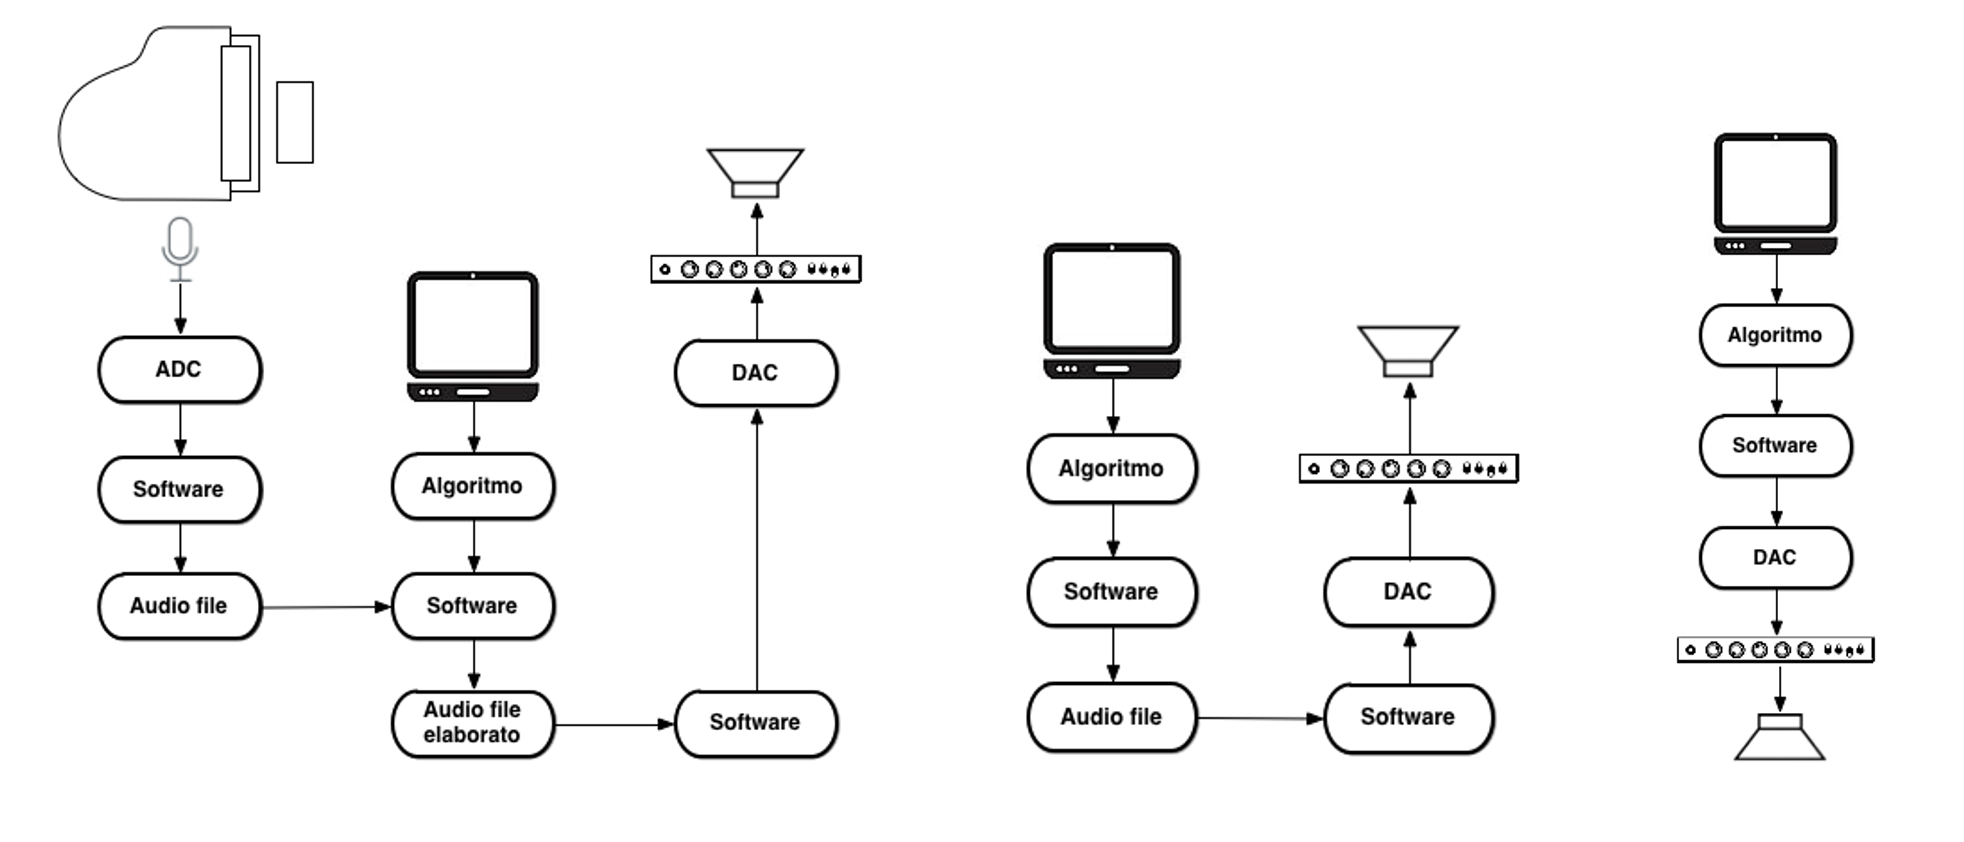
\includegraphics[scale=1]{../img/chains.png}
\end{center}

\subsection{Fixed media music }\label{fixed-media-music}

This subcategory denotes music or video that is played back from a recording.

This used to be called `tape music' but tapes are no longer used.

The entire work is stored on a single medium and reproduced from beginning to end.

We can identify three main genres:

\begin{itemize}
\tightlist
\item acousmatic music.
\item wallpaper music, ambient music and soundscapes.
\item radiodrama.
\end{itemize}

\subsubsection{Acousmatic music }\label{acousmatic-music}

\begin{center}
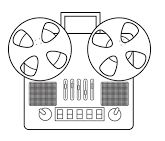
\includegraphics[scale=0.5]{../img/tape.png}
\end{center}

We can start from \textit{musique concrète}.

In the 1940s Pierre Schaeffer began composing with the sound (acoustic world).

After applying various sound elaborations (editing, filtering, reversal, etc.) he began to apply musical techniques to their combinations (repetition, transposition, reordering, etc.) inventing new musical structures (symbolic world).

In doing so, he reversed the compositional practice that had been in force for centuries in the Western musical tradition.

The listeners could not make the cognitive associations illustrated in the first chapter.

They activating exclusively the basic cognitive mechanisms common to all human beings.

This listening mode has been called \textit{reduced listening}.

All listeners of this new music are comparable to the aborigine who listens to a Beethoven symphony.

P.Shaeffer - \href{http://www.musicaecodice.it/gitmedia/emc/2_media/shaeffer.mp3}{Etude aux chemins de fer} for tape (1948) - extract.

\begin{itemize}
\tightlist
\item mono analog tape.
\item recorded and processed train sounds.
\item sounds from the acoustic environment.
\item we can recognize the sound source and its processing.
\item perceived as a distortion of reality.
\end{itemize}

Acousmatic music is the modern evolution of musique concrète.

By the mid-1970s a number of composers felt a need to designate their conception clearly in terms of specific methodology, syntax, and tools.

François Bayle suggested adopting the term acousmatique.

This term comes from the Greekakousma: what is heard.

Students of Pythagoras listened to his teachings from behind a screen unable to see him.

He believed that the lack of visual cues would force his students to focus all their attention on his message.

After his death his followers split into:

\begin{itemize}
\tightlist
\item acousmatics (practitioners of the mystic doctrine)
\item mathematics (scientists).
\end{itemize}

The loudspeaker was the modern equivalent of the screen partition.

\textit{"From an esthetical point of view acousmatic music concentrates on the poetical and spectral richness of sounds, and plays with this very particular characteristic of sound hearing in which the perception of anacoustic phenomena is associated with its cause; hence the perception of a sound whose cause is unknown or unrecognizable for our perception, induces the listener to imagine non-existing causes and to perceive
music as a complex creative phenomena in which musical sense and musical sounds have to be interpreted simultaneously, with generally very little relation with our perceptive reality. The question is not to find out how sounds are made but how their combination will generate imaginary perceptions of imaginary realities in our mind."}

Teruggi, D. 1995. What about acousmatics? In Journal of Electroacoustic
Music. Vol. 7. London: Sonic Arts Network

\href{http://www.musicaecodice.it/gitmedia/emc/2_media/teruggi.pdf}{More info}

B.Parmegiani - \href{http://www.musicaecodice.it/gitmedia/emc/2_media/parmegiani.mp3}{De Natura Sonorum} for tape (1975) - extract.

\begin{itemize}
\tightlist
\item stereo digital tape.
\item recorded and processed sounds plus synthetic sounds.
\item sounds from an imaginary environment.
\item we cannot recognize the sound source.
\item perceived as an alternative or virtual reality.
\end{itemize}

Another characteristic of acousmatic music is that it is performed live on loudspeaker orchestras (acousmonium).

Indeed Bayle referred to acousmatic musica as \textit{"art of projected sounds which is shot and developed in the studio, projected in a hall, like cinema".}

H.Vaggione - \href{http://www.musicaecodice.it/gitmedia/emc/2_media/vaggione.mp3}{Consort}. for convolved violins (2011) - extract.

\begin{itemize}
\tightlist
\item multitrack digital file.
\item recorded and processed instrumental sounds.
\item sounds from music environment.
\item we can recognize the sound source and its avatars.
\item perceived as a piece of music.
\end{itemize}

\href{http://www.musicaecodice.it/gitmedia/emc/2_media/space.pdf}{More info} about acousmatic works interpretation.

\subsubsection{Wallpaper music, ambient music and soundscapes }\label{wallpaper-music-ambient-music-and-soundscapes}

\begin{center}
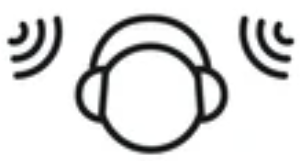
\includegraphics[scale=0.4]{../img/ambi.png}
\end{center}

We can start from Eric Satie (non-electroacoustic composer).

He was a precursor of minimalism, muzak, and many other 20th-century musical genres.

Satie conceived this musical genre as a backdrop to everyday activities (passive listening).

Satie was familiar with this idea due to its role as role as a Montmartre café pianist in the late 19th and early 20th century.

E.Satie - \href{http://www.musicaecodice.it/gitmedia/emc/2_media/satie.mp3}{Musique d'ameublement} (1917) for ensemble - extract.

\begin{itemize}
\tightlist
\item acoustic instruments.
\item pattern iteration.
\item music environment.
\item time dilation (psychological time).
\item passive and non immersive listening.
\item perceived as a piece of music.
\end{itemize}

We know well how nowadays we are bombarded daily by this type of music in a totally involuntary motion.

Let us recall what was stated in the first chapter on the basic cognitive mechanisms of human beings.

In the 1950s a visionary composer like J.Cage took this idea to its extreme with the piece 4'33'\,' whose sonic and musical content consists of the background noise of a finite time.

Later in 1978 another composer Brian Eno coined the term ambient as a musical genre.

A Sunday morning in the Cologne airport while waiting for a flight he tought: \textit{The light was beautiful, everything was beautiful, except they were playing awful music. They spend hundreds of millions of pounds\ldots on everything. Except the music.}

It was this that compelled him to begin composing music for public environments.

We must consider that the diffusion of sounds and/or music in environments not designed for active listening can change the perception of that environment in a subconscious way.

It is time that through sound redraws the boundaries of a space.

B.Eno - \href{http://www.musicaecodice.it/gitmedia/emc/2_media/eno.mp3}{Music for Airports} (1978) for tape - extract.

\begin{itemize}
\tightlist
\item stereo vynil. 
\item pattern iteration.
\item music environment. 
\item time dilation (psychological time). 
\item passive and semi immersive listening. 
\item perceived as a piece of music.
\end{itemize}

\href{http://www.musicaecodice.it/gitmedia/emc/2_media/eno.pdf}{More info}

Soundscape composition can represent a meeting point between musique concrete and ambient music because:

\begin{itemize}
\tightlist
\item it uses sound materials recorded from the real world or synthesized.
\item does not recompose them according to symbolic rules and principles into a musical form.
\item its purpose is to construct or reconstruct a real or virtual soundscape.
\end{itemize}

It's essentially based on the studies and works of Canadian musicologist and composer Raymond Murray Schafer.

To put it simply, we can say that different types of sounds coexist in a sound environment and we can identify three types:

\begin{itemize}
\tightlist
\item geophony \(\rightarrow\) all the sounds of nature of non-biological origin.
\item biophony \(\rightarrow\) all the sounds of nature of biological origin but not caused by humans.
\item anthrophony \(\rightarrow\) all sounds generated by humans.
  \begin{itemize}
  \tightlist
  \item language.
  \item music.
  \item mechanical sound.
  \end{itemize}
\end{itemize}

Schafer also divides the sounds of a soundscape into two categories:

\begin{itemize}
\tightlist
\item hi-fi \(\rightarrow\) all sounds that have an hight signal-to-noise ratio (they are distinguishable from the background noise).
\item lo-fi \(\rightarrow\) all sounds that have a low signal-to-noise ratio (they are indistinguishable from the background noise).
\end{itemize}

Three main elements in a soundscape:

\begin{itemize}
\tightlist
\item keynote \(\rightarrow\) sounds that most characterize an environment, analogous to the tonality in tonal music.
\item sound signals \(\rightarrow\) all the foreground sounds that do not necessarily characterize an environment but may appear occasionally.
\item soundmark \(\rightarrow\) The unique sounds of a given soundscape.
\end{itemize}

N.Barret - \href{http://www.musicaecodice.it/gitmedia/emc/2_media/soundwalk.mp3}{Soundwalk} (1998) - extract.

\begin{itemize}
\tightlist
\item stereo digital tape. 
\item no pattern. 
\item acoustic environment. 
\item time as in real life (clock time). 
\item passive and immersive listening. 
\item perceived as an acoustoc environment.
\end{itemize}

\href{http://www.musicaecodice.it/gitmedia/emc/2_media//schafer.pdf}{More info}

\subsubsection{Radiodrama }\label{radiodrama}

\begin{center}

\includegraphics[scale=0.5]{../img/radio.png}
\end{center}

Radio drama can use only four kinds of signs:

\begin{itemize}
\tightlist
\item speech.
\item sound effects.
\item music.
\item silence.
\end{itemize}

Any one of these by itself can be a very slippery client to deal with.

Silence cane a listener suspect a transmission failure and switch off or tune over to another on.

Sound effects are notoriously misleading - a sneeze can be taken for a bomb explosion!

An unfamiliar music will sound irritatingly like cacophony.

And speech says nothing to someone who doesn't know what you mean by the words.

But if you hit on harmonious combination of the right choies of these four kinds you can move mountains, deploy infantry battalions with Air Force support, immerse a soul in the joys of paradise.

In short do anything you please, all in few minutes one after another.

The main focus is narrativity and a continuous balance in the construction of meaning between explicit sounds (both in natural and auditory language) and perceptual hints and/or allusions.

O.Wells - \href{http://www.musicaecodice.it/gitmedia/emc/2_media/wells.mp3}{War of the worlds} (1938) - extract.

\begin{itemize}
\tightlist
\item mono radio signal.
\item natural language.
\item didactic sound design to simulate the real acoustic environment.
\item time as in real life (clock time).
\item active listening non immersive.
\item perceived as a representation of reality.
\end{itemize}

\href{http://www.musicaecodice.it/gitmedia/emc/2_media/radio.pdf}{More info}

\subsubsection{Computer music - algorithmic composition}\label{computer-music---algorithmic-composition}

\begin{center}

\includegraphics[scale=0.5]{../img/comp.png}
\end{center}

The birth of computer music is naturally linked to the invention of the electronic calculator and the subsequent spread of personal computers as well as the invention of new (formal) languages that allow humans to communicate with these machines.

Starting from the second half of the 1950s, two orientations emerged:

\begin{itemize}
\tightlist
\item the first one (developed mainly in Europe) deals with the digital coding of musical parameters (assisted composition, assisted musical analysis, etc.).
\item the second one (developed mainly in USA) deals with the digital coding of sound parameters (synthesis and processing).
\end{itemize}

In 1957 MUSIC I was created by Max Mathews in Bell Laboratories.

It was the first software for playing music from mathematical functions.

After MUSIC I, there were: MUSIC II, III, IV, V, MUSIC 360, and then C-sound and SuperCollider languages still used today.

The main sound synthesis and processing techniques used are:

\begin{itemize}
\tightlist
\item additive synthesis.
\item subctractive synthesis (filters).
\item FM (Frequency Modulation) synthesis.
\item granular synthesis.
\item analysis and resynthesis (FFT).
\item generative algorithms for:

  \begin{itemize} 
  \tightlist
  \item musical structures.
  \item timbres.
  \item pitches.
  \end{itemize}
\item remote control of computers (MIDI, OSC, HID).
\end{itemize}

As we all know, nowadays computer is the main musical instrument, like piano in the 19th century.

The term \textit{computer music} as an aesthetic category identifies the musical genre adopted by the pioneers from the mid-50s to the late 90s

J.Chowning - \href{http://www.musicaecodice.it/gitmedia/emc/2_media/chowning%20.mp3}{Stria}. (1977) - extract.

\begin{itemize}
\tightlist
\item stereo digital tape.
\item sonic environment.
\item sounds from imaginary environment (only synthetic sounds - FM).
\item time dilation (psychological time).
\item active listening.
\item perceived as a piece of computer music.
\end{itemize}

\href{http://www.musicaecodice.it/gitmedia/emc/2_media/max.pdf}{More info}

\subsection{Live sequencing}\label{live-sequencing}

This subcategory is almost identical to the previous one except for two aspects: 

\begin{itemize}
\tightlist
\item works can be generated in real time through algorithms (computer music). 
\item tracks are divided into different sound files triggered in real time (sound design for theatre and gaming).
\end{itemize}

\subsubsection{Sound design for performing arts or video }\label{sound-design-for-performing-arts-or-video}

\begin{center}
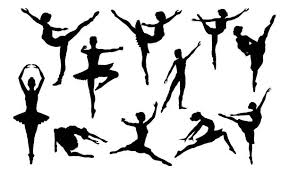
\includegraphics[scale=0.4]{../img/danza.png}
\end{center}

Works on fixed media which differ from the works illustrated in the previous section essentially for:

\begin{itemize}
\tightlist
\item sound does not have an absolute value but must be functional to dramaturgy.
\item divised into more or less short fragments.
\item open form \(\rightarrow\) fragments can be triggered in non-linear sequences (slightly different than what was said about random generation).
\item differenze musicali rispetto ai brani acusmatici.
\end{itemize}

Anonymous - \href{http://www.musicaecodice.it/gitmedia/emc/2_media/dance.mp3}{Dance!} (2010) - extract.

\begin{itemize}
\tightlist 
\item stereo digital tape. 
\item music functional to movement or dramatic timing.
\item secondary sensitive plane. 
\item passive listening. 
\item perceived as a complement to visual information.
\end{itemize}

\subsubsection{Sound design for gaming}\label{sound-design-for-gaming}

\begin{center}

\includegraphics[scale=0.3]{../img/game.png}
\end{center}

In this case too the sound must be functional to the game

It should:

\begin{itemize}
\tightlist
\item suggest a mood, evoke a feeling.
\item indicate a geographical locale.
\item define a character.
\item mirror or exaggerate how things sound in real life.
\item clarify the narrative
\end{itemize}

To simplify there are five sounds categories:

\begin{itemize}
\tightlist
\item dialogue \(\rightarrow\) any verbal speech in the game (player talk).
\item music \(\rightarrow\) any non-diegetic music (orchestral music).
\item sound Effects (Hard Effects) \(\rightarrow\) any sound from an real-life object (sounds of rocks falling).
\item foley \(\rightarrow\) any sound effect that the player makes (footsteps, etc.).
\item backgrounds (ambience) \(\rightarrow\) noise from the environment (wind, rain, etc.).
\end{itemize}

Procedural audio:

\begin{itemize}
\tightlist
\item sounfiles triggered by user actions.
\item real time shynthesis by internal oscillators.
\end{itemize}

Artistically we could merge game music, soundscape composition, acousmatic music and radiodrama.

Various - \href{http://www.musicaecodice.it/gitmedia/emc/2_media/gaming.mp3}{8 bit music}(1990) - extracts.

\begin{itemize}
\tightlist
\item stereo digital samples or real time oscillators.
\item music functional to gamer emotions.
\item also called procedural music.
\item pattern iteration.
\item music environment.
\item time dilation (psychological time).
\item non-immersive audio diffusion but immersive psychological function.
\item passive listening.
\end{itemize}

\href{http://www.musicaecodice.it/gitmedia/emc/2_media/gaming.pdf}{More info}

\section{Interactive systems }\label{interactive-systems}

This category includes genres that:

\begin{itemize}
\tightlist
\item involve human interaction during the performance as happens with acoustic instruments.
\item these interactions influence the musical or sound text at different levels.
\end{itemize}

Compared to the previous typology the presence of one or more performers significantly influences:

\begin{itemize}
\tightlist
\item the anthropological and contextualised perception of the musical action.
\item its representative nature.
\end{itemize}

This category can be divided into three further subcategories:

\begin{itemize}
\tightlist
\item hyper-instruments.
\item live set.
\item live coding.
\end{itemize}

The image shows the possibles audio chains in this category.

\begin{itemize}
\tightlist
\item real-time processing of pre-recorded or pre-synthesized sounds (parameters can be controlled through various types of devices - MIDI, OSC, HID, sensors).
\item real-time processing of signals captured through microphones or sensors (parameters can be controlled (parameters can be controlled in the previous modes but also through control signals derived in some way from the incoming audio signal).
\end{itemize}

\begin{center}
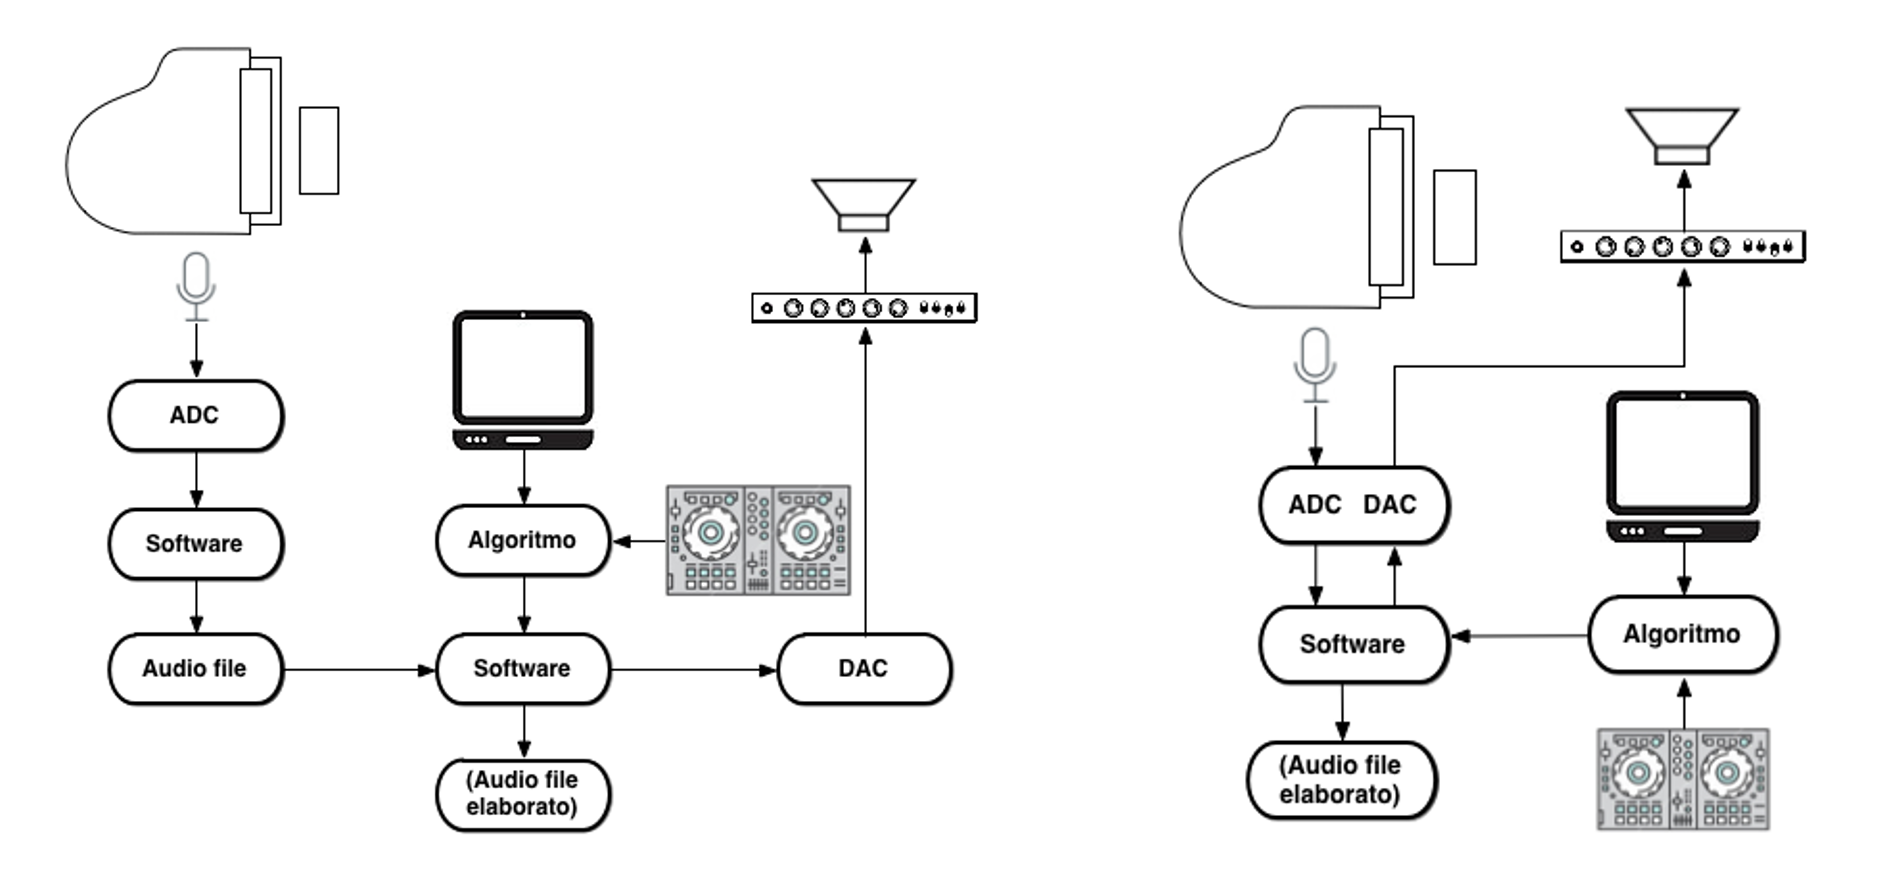
\includegraphics[scale=1]{../img/chain2.png}
\end{center}

\subsection{Hyper-instrument}\label{hyper-instrument}

\begin{center}

\includegraphics[scale=0.6]{../img/lel.png}\\
P.Boulez - \href{http://www.musicaecodice.it/gitmedia/emc/2_media/boulez1.mp4}{Anthèmes 2} (1994) - extract.
\end{center}

Augmented musical instrument that uses technology to extend the capabilities of a traditional instrument and enhance the performer's expressiveness.

Two types:

\begin{itemize}
\tightlist
\item real-time augmented instrumental techniques \(\rightarrow\) sound processes are controlled by:

  \begin{itemize}
  \tightlist
  \item an electronic performer who interacts with different types of controllers.
  \item by information extracted from the audio signal produced by the instrument itself (feature extraction as control signals).
  \end{itemize}
\item cyborg luthiery \(\rightarrow\) sound processing is controlled by movements and/or gestures of the performer captured by different types of sensors.
\end{itemize}

Three main goals:

\begin{itemize}
\tightlist
\item respond to the performer's input in a dynamic and expressive way allowing for a deeper connection between the musician and the music.
\item produce sounds and musical effects that are impossible to achieve with traditional instruments alone.
\item expanding musical forms.
\end{itemize}

\subsection{Live set }\label{live-set}

\begin{center}
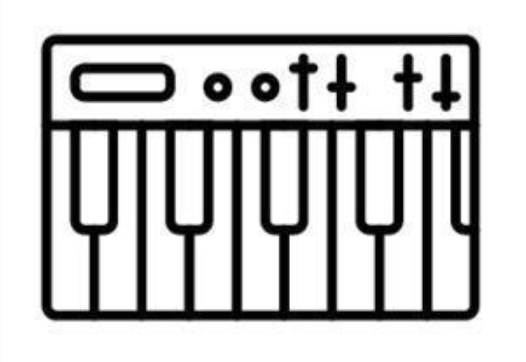
\includegraphics[scale=0.3]{../img/lset.png}\\
Slork - \href{http://www.musicaecodice.it/gitmedia/emc/2_media/slork1.mp4}{Twilight} (2013) - extract.
\end{center}

Live performance where songs are performed using analog or digital electronic musical instruments.

Often musicians improvise in a live set, making each performance unique.

Can be a solo performance or a laptop ensemble.

One of the most important aspects of this genre is to think about and assemble original performance environments which leads to the search for new human/machine interfaces dedicated to the generation of new sounds in the musical field.

\subsection{Live coding}\label{live-coding}

\begin{center}

\includegraphics[scale=0.4]{../img/lcod.png}\\
SuperCollider \href{http://www.musicaecodice.it/gitmedia/emc/2_media/livec1.mp4}{Live Coding} - extract.
\end{center}

Also called:

\begin{itemize}
\tightlist
\item on-the-fly programming.
\item just in time programming.
\item conversational programming.
\end{itemize}

Search for new musical forms, new places for performance and new audiences.

It is part of a larger artistic movement called creative coding.

If channeled into the Western musical tradition, we can think of it as a new version of organ improvisations in the Baroque era.

From a semiographic point of view the most interesting aspect is that the score is the code and is created and manipulated in real time.

The compositional process which has always belonged to the author's private sphere becomes public and an integral part of the performance itself (do you remember the first paragraphs of the previous chapter?).

\section{The virtual instrument paradigm}\label{the-virtual-instrument-paradigm}

In this section we define a virtual instrument model that will be useful in next chapters.

If anyone is unfamiliar with SuperCollider, they can download an introductory text at
\href{https://ccrma.stanford.edu/~ruviaro/texts/A_Gentle_Introduction_To_SuperCollider.pdf}{this
link}.

In the chapter on live electronics we'll make some small modifications to allow signal input.

\subsection{Software installation }\label{software-installation}

Download and install:

\begin{itemize}
\tightlist
\item \href{https://github.com/capital-G/sc_kernel}{sc\_kernel} (if you want to execute supercollider code in this notebook)
\item \href{https://supercollider.github.io/}{SuperCollider}
\end{itemize}

If you want to play SuperCollider from this notebook you have to select the textit{sc\_kernel}.

Instead, I recommend copying and pasting the code into the SuperCollider IDE Interpreter.

\subsection{Instrumental model}\label{instrumental-model}

Let's create a computer model that contains functions common to most virtual instruments (sound generators).

\begin{itemize}
\tightlist
\item an oscillator.
\item an amplitude envelope (with or without sustain).
\item a stereo panner.
\item a signal output.
\end{itemize}

We also establish the basic parameters we want to control dynamically (they will increase depending on the synthesis algorithm chosen).

\begin{itemize}
\tightlist
\item frequency (Hz).
\item general amplitude (0.0 to 1.0).
\item duration (seconds).
\item pan position (-1.0 to +1-0).
\item pan interpolation time (movements)
\item output bus.
\item trigger.
\item kind of voice allocation (doneAction:0 or 2).
\end{itemize}

\begin{center}
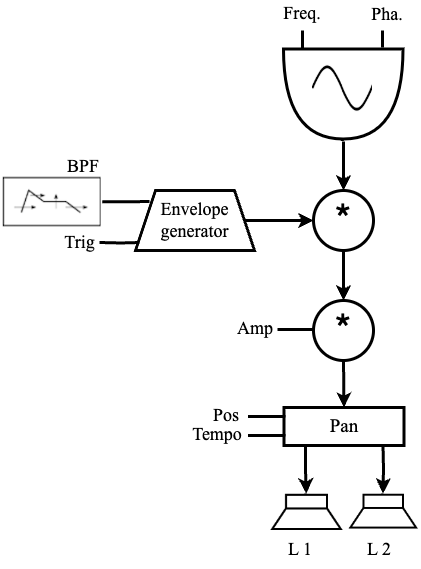
\includegraphics[scale=0.35]{../img/modello.png}
\end{center}

\begin{lstlisting}[frame=single] 
s.boot;
s.meter;
s.scope;
s.plotTree;
\end{lstlisting}

In SuperCollider we can define it with the `SynthDef' (synthesis definition) class.

This class contains the instructions (algorithms) needed to build multiple copies (instances) derived from the model.

\begin{lstlisting}[frame=single, caption=Instrument model] 
SynthDef.new(\model, {arg freq=500, amp=0, dur=1, pan=0, pantime(0.0), 
                          out=0, t_gate=0, done=2;
                      var sig, env;
                          sig = SinOsc.ar(freq);
                          env = Env.new([0.0,1.0,0.5,0.7,0],                
                                        [0.1,0.1,0.3,1.0].normalizeSum * dur,
                                        -4    
                                        );
                          env = EnvGen.kr(env, t_gate, doneAction:done);
                          sig = sig * env * amp;
                          sig = Pan2.ar(sig, pan.varlag(pantime));
                      Out.ar(out, sig)
                      }).add;        
\end{lstlisting}
Now we can generate as many instances as we want.

We have two ways to control the instance parameters.

They vary depending on the voice allocation we want.

\textbf{Dynamic voice allocation (poliphonic)} 

Instance self-destructs when the amplitude envelope expires (doneAction:2).

In this case we pass parameters at instantiation time (array of \textbackslash key, value).

\begin{lstlisting}[frame=single,caption=Dynamic voice allocation] 
Synth.new(\model, [\freq, rrand(890,1234), 
                   \amp, 0.5, 
                   \dur, rrand(0.1,2), 
                   \pan, rand2(1.0), 
                   \pantime, 0.1, 
                   \done, 2, 
                   \t_gate,1 ])
\end{lstlisting}

\textbf{Static voice allocation (monophnic)}

Two passages: 

\begin{itemize}
\tightlist
\item create instance and assign it to a variable.
\item send one or multiple parameter changes by \textit{set} method.

\begin{lstlisting}[frame=single, caption=Static voice allocation] 
a = Synth.new(\model, [\done, 0]);
a.set(\freq, rrand(890,1234), 
      \amp, 0.5, 
      \dur, rrand(0.1,2), 
      \pan, rand2(1.0), 
      \pantime, 0.1, 
      \t_gate,1)
\end{lstlisting}
\end{itemize}

Then we can kill it.

\begin{lstlisting}[frame=single] 
a.free;
\end{lstlisting}
Or kill all Synths on the Server.

\begin{lstlisting}[frame=single] 
s.freeAll;
\end{lstlisting}
The type of voice allocation is strictly linked to the type of amplitude envelope.

\textbf{With sustain (as in keyboards)}

There isn't a total duration.

In this case we must send a message of \textit{gate 1} (noteon) and then textit{gate 0} (noteoff).

\begin{lstlisting}[frame=single, caption=Instrument model with sustain] 
SynthDef.new(\sust, {arg freq=500, amp=0, pan=0, pantime(0.0), 
                     out=0, gate=0, done=2;
                     var sig, env;
                         sig = SinOsc.ar(freq);
                         env = Env.adsr;         
                         env = EnvGen.kr(env, gate, doneAction:done);
                         sig = sig * env * amp;
                         sig = Pan2.ar(sig, 0);
                     Out.ar(0, sig)
                     }).add;       
                                                
a = Synth.new(\sust, [\done, 0]); 
\end{lstlisting}
Send \textit{gate 1} (noteon)
\begin{lstlisting}[frame=single] 
a.set(\amp, 0.5, \gate, 1);
\end{lstlisting}
Send \textit{gate 0} (noteoff)
\begin{lstlisting}[frame=single] 
a.set(\gate, 0);
\end{lstlisting}
Kill the Synth.
\begin{lstlisting}[frame=single] 
a.free;
\end{lstlisting}

\textbf{Without sustain (as in percussion or plucked intruments)}

There is a total duration.

In this case we must send a gate message preceded by \textit{t\_}.

This produce an automatic \textit{gate 0} message after a time calculated on the specified duration

\begin{lstlisting}[frame=single, caption=Instrument model without sustain] 
SynthDef.new(\nosust,  {arg freq=500, amp=0, dur=1, pan=0, pantime(0.0), 
                            out=0, t_gate=0, done=2;
                        var sig, env;
                            sig = SinOsc.ar(freq);
                            env = Env.perc(0.1*dur,0.9*dur);                     
                            env = EnvGen.kr(env, t_gate, doneAction:done);
                            sig = sig * env * amp;
                            sig = Pan2.ar(sig, 0);
                        Out.ar(0, sig)
                        }).add;                                                   
a = Synth.new(\nosust, [\done, 0]);    // Create the Synth
\end{lstlisting}

Send \textit{t\_gate 1} (noteon + noteoff)

\begin{lstlisting}[frame=single] 
a.set(\amp, 0.5, \t_gate,1);
\end{lstlisting}

You can also trigger and kill it automatically.

\begin{lstlisting}[frame=single] 
a.set(\amp, 0.5, \done, 2, \t_gate,1);
\end{lstlisting}

Modifications to this model will be addressed in specific chapters.